% $Header: /Users/joseph/Documents/LaTeX/beamer/solutions/conference-talks/conference-ornate-20min.en.tex,v 90e850259b8b 2007/01/28 20:48:30 tantau $

\documentclass[utf8,t,compress,xcolor=svgnames,handout]{beamer}

\usepackage{pgfpages}
\pgfpagesuselayout{4 on 1}[a4paper,landscape,border shrink=5mm]

\usepackage{calc}
\usepackage{ifthen}
\usepackage[sfdefault]{cabin}
\usepackage[T1]{fontenc}
\usepackage[english]{babel}	   % English hyphenation
\usepackage{csquotes}		 % Multilingual quotes
\usepackage[babel]{microtype}    % Awesome microtyping

\usepackage{booktabs}    % Better tables
%\usepackage{tablefootnote}    % Allows footnotes in tables
\usepackage{commath}    % Differential operators
\usepackage{bm}
\usepackage{multirow}

% Extra symbols
\usepackage{wasysym}
\newcommand\pro{\item[\textbf{\CheckedBox}]}
\newcommand\con{\item[\textbf{\XBox}]}
\newcommand\neu{\item[\textbf{\Square}]}

% Graphics
\usepackage{graphicx}
\DeclareGraphicsExtensions{.pdf,.png,.jpg}
\graphicspath{{img/}}    % Central repository for images
\usepackage{emerald}
\usepackage{tikz}
\usepackage{pgf}
\usepackage{pgffor}
\usepackage{mathrsfs}
\usetikzlibrary{arrows,shapes.geometric,shapes.misc}

% Bibliography
\usepackage[backend=biber,style=alphabetic,sorting=ydnt]{biblatex}
\addbibresource{thesis.bib}

% Set fonts
\setbeamerfont{my frametitle}{size=\Large}
\setbeamerfont{framesubtitle}{size=\large}
\setbeamerfont{title}{size=\huge}
\setbeamerfont{subtitle}{size=\Large}
\setbeamerfont{author}{size=\large}
\setbeamerfont{date}{size=\large}
\setbeamerfont{institute}{size=\large}

%%% Frametitle
%\setbeamertemplate{frametitle}{
%	\begin{beamercolorbox}{frametitle}
%		\vskip0.75em
%		\usebeamerfont{frametitle}
%		\insertframetitle \\
%		\usebeamerfont{framesubtitle}\insertframesubtitle
%	\end{beamercolorbox}
%}
%
%%% remove navigation symbols
%\setbeamertemplate{navigation symbols}{}
%
%%% Date in the Corner
%\setbeamertemplate{headline}{
%	\rotatebox{30}{
%		\ifx\insertdate\empty\else        
%		\hspace*{0.25cm}\insertshortdate\hspace*{0.5cm}
%		\fi
%	}
%	\vspace*{-1cm}
%}


% Figure styles
\tikzset{
	header/.style={
		% The shape:
		rectangle,minimum size=6mm,
		% The rest
		draw=black!10,
	}}
	
	\tikzset{
		term/.style={
			% The shape:
			shape=rectangle,rounded corners=3mm,
			% The size:
			minimum size=6mm,
			% The border:
			very thick,
			draw=red!50!black!50, % 50% red and 50% black,
			% and that mixed with 50% white
			% The filling:
			%			top color=white, % a shading that is white at the top...
			%			bottom color=red!50!black!20 % and something else at the bottom
		}}
		
		\tikzset{
			nterm/.style={
				% The shape:
				rectangle,minimum size=6mm,rounded corners=3mm,
				% The rest
				very thick,draw=black!30,
				%			top color=black!05,bottom color=black!10,
			}}
			
			
			\title{Pricing exotic path-dependent options}
			\subtitle{The Singular Points method}
			\date[2015-10-23]{23\textsuperscript{rd} October, 2015}
			\institute[MathMods]{MathMods\\{Universita degli Studi dell'Aquila}}
			\author[Sudip Sinha]{Sudip Sinha}

% This file is a solution template for:

% - Talk at a conference/colloquium.
% - Talk length is about 20min.
% - Style is ornate.



% Copyright 2004 by Till Tantau <tantau@users.sourceforge.net>.
%
% In principle, this file can be redistributed and/or modified under
% the terms of the GNU Public License, version 2.
%
% However, this file is supposed to be a template to be modified
% for your own needs. For this reason, if you use this file as a
% template and not specifically distribute it as part of a another
% package/program, I grant the extra permission to freely copy and
% modify this file as you see fit and even to delete this copyright
% notice. 


\mode<presentation>
{
  \usetheme{Warsaw}
  % or ...

  \setbeamercovered{transparent}
  % or whatever (possibly just delete it)
}



\title{Pricing exotic path-dependent options}
\subtitle{The Singular Points method}
\date[2015-10-23]{23\textsuperscript{rd} October, 2015}
\institute[MathMods]{MathMods\\{Università degli Studi dell'Aquila}}
\author[Sudip Sinha]{Sudip Sinha\\{Supervisor: Prof. Fabio Antonelli}}
\subject{Mathematical Finance}



% If you have a file called "university-logo-filename.xxx", where xxx
% is a graphic format that can be processed by latex or pdflatex,
% resp., then you can add a logo as follows:

% \pgfdeclareimage[height=0.5cm]{university-logo}{university-logo-filename}
% \logo{\pgfuseimage{university-logo}}



% Delete this, if you do not want the table of contents to pop up at
% the beginning of each subsection:
\AtBeginSubsection[]
{
  \begin{frame}<beamer>{Outline}
    \tableofcontents[currentsection,currentsubsection]
  \end{frame}
}


% If you wish to uncover everything in a step-wise fashion, uncomment
% the following command: 

%\beamerdefaultoverlayspecification{<+->}


\begin{document}
	
	\begin{frame}[plain]
		\maketitle
	\end{frame}
	
	
	\section{Motivation}
	
	\begin{frame}{Introduction}
		\begin{itemize}
			
			\item Assets
			\begin{itemize}
				\item basic assets
				\begin{description}
					\item[riskless] deterministic: $ S_t^0 = e^{rt} $
					\item[risky] stochastic process: $ (S_t)_t $
				\end{description}
				\item derivatives -- contracts on other assets
				\begin{description}
					\item[futures \& forwards] symmetric risk
					\item[options] asymmetric risk
				\end{description}			
			\end{itemize}
			
			\item Problem: pricing derivatives -- finding a fair price
			
			\item Assumptions
			\begin{itemize}
				\item viable / no arbitrage / no free lunch
				\item frictionless
				\item infinitely divisible assets
			\end{itemize}
		\end{itemize}
		
	\end{frame}
	
	
	\begin{frame}{Option types}
		\begin{itemize}
			\item Simple options -- classification of the basis of:
			\begin{description}
				\item[exercise time] European or American
				\item[right of owner] call or put
			\end{description}
			\begin{example}[European call]
				payoff function: $ (S_T - K)_+ = \max \{S_T - K, 0\} $, exercise only at maturity
			\end{example}
			\item Exotic options
			\begin{description}
				\item[\alert{Asian}] payoff: function of average of the underlying.
				\item[lookback] payoff: function of extrema of the underlying.
				\item[\alert{cliquet}] A series of globally or locally, capped or floored, at-the-money options.
				\item[digital] existence depends on pre-set barriers.
			\end{description}
		\end{itemize}
	\end{frame}
	
	
	%	notes: recombinant; n = 3; same outcome; two different paths => different averages
	\begin{frame}{Visual representation of risky asset}
		\begin{figure}
			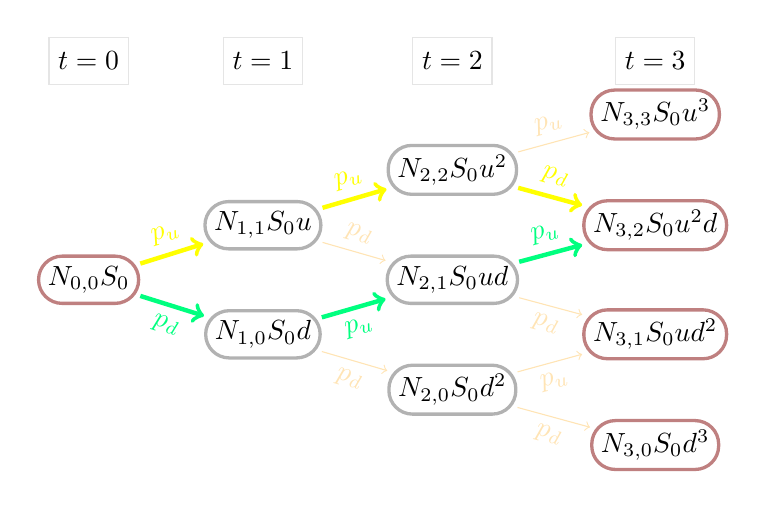
\begin{tikzpicture}
			\matrix[column sep=8mm,row sep=0.4mm,ampersand replacement=\&] (tree){
				\node[header] (t0) {$ t = 0 $};  \&  \node[header] (t1) {$ t = 1 $};  \&  \node[header] (t2) {$ t = 2 $};  \&  \node[header] (t3) {$ t = 3 $};  \\
				\&  \&  \& \node[term] (u3) {$ N_{3,3} \blacktriangleright S_0 u^3 $};  \\
				\&  \&  \node[nterm] (u2) {$ N_{2,2} \blacktriangleright S_0 u^2 $};  \&  \\
				\&  \node[nterm] (u) {$ N_{1,1} \blacktriangleright S_0 u $};  \&  \&  \node[term] (u2d) {$ N_{3,2} \blacktriangleright S_0 u^2 d $};  \\
				\node[term] (s) {$ N_{0,0} \blacktriangleright S_0 $};  \&  \&  \node[nterm] (ud) {$ N_{2,1} \blacktriangleright S_0 u d $};  \&  \\
				\&  \node[nterm] (d) {$ N_{1,0} \blacktriangleright S_0 d $};  \&  \&	\node[term] (ud2) {$ N_{3,1} \blacktriangleright S_0 u d^2 $};  \\
				\&  \&  \node[nterm] (d2) {$ N_{2,0} \blacktriangleright S_0 d^2 $};  \&  \\
				\&  \&  \& \node[term] (d3) {$ N_{3,0} \blacktriangleright S_0 d^3 $};  \\
			};
			
			% Lines out of s
			\draw[->,Yellow,ultra thick] (s) -- (u) node[midway,above,sloped] {$p_u$};
			\draw[->,SpringGreen,ultra thick] (s) -- (d) node[midway,below,sloped] {$p_d$};
			% Lines out of u
			\draw[->,Yellow,ultra thick] (u) -- (u2) node[midway,above,sloped] {$p_u$};
			\draw[->,Moccasin] (u) -- (ud) node[midway,above,sloped] {$p_d$};
			% Lines out of d
			\draw[->,SpringGreen,ultra thick] (d) -- (ud) node[midway,below,sloped] {$p_u$};
			\draw[->,Moccasin] (d) -- (d2) node[midway,below,sloped] {$p_d$};
			% Lines out of u2
			\draw[->,Moccasin] (u2) -- (u3) node[midway,above,sloped] {$p_u$};
			\draw[->,Yellow,ultra thick] (u2) -- (u2d) node[midway,above,sloped] {$p_d$};
			% Lines out of ud
			\draw[->,SpringGreen,ultra thick] (ud) -- (u2d) node[midway,above,sloped] {$p_u$};
			\draw[->,Moccasin] (ud) -- (ud2) node[midway,below,sloped] {$p_d$};
			% Lines out of d2
			\draw[->,Moccasin] (d2) -- (ud2) node[midway,below,sloped] {$p_u$};
			\draw[->,Moccasin] (d2) -- (d3) node[midway,below,sloped] {$p_d$};
			\end{tikzpicture}
			
			%		\caption{A 3-step recombinant tree}
			%		\label{fig:paths}
		\end{figure}
	\end{frame}
	
	
	\begin{frame}{Market models -- discrete vs continuous}
		\begin{tabular}{lll}
			\toprule
			Parameter  &  Discrete  &  Continuous  \\
			\midrule
			Example  &  \cite{Cox1979}  &  \cite{Black1973}  \\
			Theoretical complexity  &  Easy  &  Hard  \\
			Ease of implementation  &  Hard  &  Easy  \\
			Closed-form formula  &  No\footnotemark  &  Yes  \\
			Computational complexity  &  Hard: $ O(2^n) $\footnotemark[1]  &  Easy: $ O(1) $  \\
			Universality  &  Yes  &  No  \\
			\bottomrule
		\end{tabular}
		\footnotetext{CRR: backward recursive}
		
		\begin{theorem}[Convergence in distribution of CRR to BS]
			CRR $ \xrightarrow{d} BS $
		\end{theorem}
		
		\alert{Quest}: Find algorithms with reduced computational complexity under discrete models converging to continuous ones.
	\end{frame}
	
	
	
	\section{Asian options}
	
	
	\begin{frame}{Asian options}{Introduction}
		\begin{definition}[Asian options]
			Payoff is a function of some form of averaging on the underlying's price.
		\end{definition}
		
		\begin{example}[fixed-strike Asian call of European type]
			A fixed-strike Asian call of European type, with a strike-price $ K $ would imply that the payoff at maturity is given by $ (A_T - K)_+ $, and the owner of the option may only exercise it at maturity.
		\end{example}
		
		\begin{tabular}{lll}
			\toprule
			Average  &  Discrete  &  Continuous  \\
			\midrule
			AM  &  $ A_n = \frac{1}{n+1} \sum_{i=0}^{n} S_n $  &  $ A_T = \frac{1}{T} \int_{0}^{T} S_t \dif t $  \\
			GM  &  $ G_n = \left( \prod_{i=0}^{n} S_n \right)^{\frac{1}{n+1}} $  &  $  
			G_T = \exp \left(  \frac{1}{T} \int_{0}^{T} \log(S_t) \dif t  \right) $  \\
			\bottomrule
		\end{tabular}
		
	\end{frame}
	
	
	\begin{frame}{Asian option}{Pre-existing methods}
		\begin{block}{Arithmetic mean}
			\begin{tabular}{cccl}
				\toprule
				Method  &  Type  &  Complex  &  Remarks  \\
				\midrule
				\cite{Cox1979}  &  Tree  &  \alert{$ O(2^n) $}  &  simple, accurate, convergence  \\
				\cite{Hull1993}  &  Tree  &  $ O(n^3) $  &  accuracy \& convergence problems  \\
				\cite{Barraquand1996}  &  Tree  &  $ O(n^3) $  &  accuracy \& convergence problems  \\
				\cite{Chalasani1999}  &  Tree  &  $ O(n^4) $  &  thin bounds, very large memory  \\
				\cite{Vecer2001}  &  PDE  &  $ O(n^2) $  &  not universally applicable  \\
				\cite{dHalluin2005}  &  PDE  &    &  more general than \cite{Vecer2001} \\
				\bottomrule
			\end{tabular}
		\end{block}
		
		\begin{block}{Geometric mean}
			Closed-form formula exist under BS.
		\end{block}
	\end{frame}
	
	
	\begin{frame}{Singular points method for Asian options}{Introduction}
		Idea: At any node $ N_{i,j} $:
		\begin{itemize}
			\item payoff $ P $: continuous, convex function of the underlying's average $ A $
			\item number of possible averages = number of paths to $ N_{i,j} $ = $ \binom{i}{j} $
			\item these averages completely characterise the payoff; no other payoff being possible under the given tree
			\item the above points $ ((A_{i,j}^l, P_{i,j}^l))_l $ are called \alert{singular points}
			\item payoff is represented as continuous, convex, and piecewise-linear function of the underlying's possible averages, found by joining the singular points
			\item minimum possible average $ A_{i,j}^{\min} = \frac{S_0}{i+1} \left( \frac{1 - d^{i-j+1}}{1-d} + d^{i-j} u \frac{1 - u^{j}}{1-u} \right)$
			\item maximum possible average $ A_{i,j}^{\max} = \frac{S_0}{i+1} \left( \frac{1 - u^{j+1}}{1-u} + u^{j} d \frac{1 - d^{i-j-1}}{1-d} \right) $
		\end{itemize}
	\end{frame}
	
	
	\begin{frame}{Singular points method for Asian options}{Start: at maturity ($ i = n $)}
		\begin{minipage}[t]{0.55\linewidth}
			At any node $ N_{n,j}, \exists $ three possibilities:
			\begin{enumerate}
				\item $ j \in \{ 0, n \} $: end points, only one path possible, only one singular point $ (A, (A-K)_+) $
				\item $ j \notin \{ 0, n \} $ and $ K \in \left( A_{n,j}^{\min}, A_{n,j}^{\max} \right) $: three singular points:
				\begin{enumerate}
					\item $ ( A_{n,j}^{\min} , 0 ) $
					\item $ ( K , 0 ) $
					\item $ ( A_{n,j}^{\max} , A_{n,j}^{\max} - K ) $
				\end{enumerate}
				\item $ j \notin \{ 0, n \} $ and $ K \notin \left( A_{n,j}^{\min}, A_{n,j}^{\max} \right) $: two singular points:
				\begin{enumerate}
					\item $ \left( A_{n,j}^{\min} , ( A_{n,j}^{\min} - K )_+ \right) $
					\item $ \left( A_{n,j}^{\max} , ( A_{n,j}^{\max} - K )_+ \right) $
				\end{enumerate}
			\end{enumerate}
		\end{minipage}
		\begin{minipage}[t]{0.40\linewidth}
			\begin{itemize}
				\item We discuss only the European case.
				\item The American case needs minor modifications.
			\end{itemize}
			\begin{figure}
				\definecolor{zzffzz}{rgb}{0.6,1.,0.6}
				\definecolor{bfffqq}{rgb}{0.7490196078431373,1.,0.}
				\definecolor{ffffzz}{rgb}{1.,1.,0.6}
				\definecolor{ffffff}{rgb}{1.,1.,1.}
				\begin{tikzpicture}[line cap=round,line join=round,>=triangle 45,x=1.0cm,y=1.0cm]
				\draw[->,color=ffffff] (-0.5,0.) -- (3.5,0.);
				\foreach \x in {,1.,2.,3.}
				\draw[shift={(\x,0)},color=ffffff] (0pt,2pt) -- (0pt,-2pt);
				\draw[color=ffffff] (3.2339019240538707,0.05820970293171456) node [anchor=south west] { A};
				\draw[->,color=ffffff] (0.,-0.5) -- (0.,2.5);
				\foreach \y in {,1.,2.}
				\draw[shift={(0,\y)},color=ffffff] (2pt,0pt) -- (-2pt,0pt);
				\draw[color=ffffff] (0.0727621286646436,2.255161943734117) node [anchor=west] { P};
				\clip(-0.5,-0.5) rectangle (3.5,2.5);
				\draw [line width=2.pt,color=bfffqq] (1.5167156875682812,0.)-- (3.,1.5);
				\draw [line width=0.4pt,dash pattern=on 2pt off 2pt,color=ffffzz] (3.,1.5)-- (3.,0.);
				\draw [line width=2.pt,color=bfffqq] (0.49804588626327045,0.)-- (1.5167156875682812,0.);
				\draw [line width=0.4pt,dash pattern=on 2pt off 2pt,color=ffffzz] (3.,1.5)-- (0.,1.4984358056218274);
				\begin{scriptsize}
				\draw [fill=ffffzz] (1.5167156875682812,0.) circle (2.5pt);
				\draw[color=ffffzz] (1.5167156875682817,-0.3642746881930386) node {$K$};
				\draw [fill=ffffzz] (3.,1.5) circle (2.5pt);
				\draw [fill=ffffzz] (3.,0.) circle (1.5pt);
				\draw[color=ffffzz] (3.0156155380599396,-0.3060649852613241) node {$A_{i,j}^{\max}$};
				\draw [fill=ffffzz] (0.49804588626327045,0.) circle (2.5pt);
				\draw[color=ffffzz] (0.6290177178596299,-0.32061741099425267) node {$A_{i,j}^{\min}$};
				\draw [fill=zzffzz] (0.,1.4984358056218274) circle (2.5pt);
				\draw[color=zzffzz] (0.8618565295864893,1.2510445681620406) node {$\left( A_{i,j}^{\max} - K \right)_+$};
				\end{scriptsize}
				\end{tikzpicture}
				
				\caption{Case 2}
			\end{figure}
			
		\end{minipage}
	\end{frame}
	
	
	\begin{frame}{Singular points method for Asian options}{Up movement at node $ N_{i,j}, \  \forall i < n $}
		\begin{minipage}[t]{0.6\linewidth}
			\begin{enumerate}
				\item Take a singular point $ A_{i+1,j}^l $.
				\item $ B^l = \frac{ ( i+2) A_{i+1,j}^l - S_{i+1,j} }{ i+1 } $.
				\item Each $ B^l \in \left[ A_{i,j}^{\min}, A_{i,j}^{\max} \right] $ is a singular average of $ N_{i,j} $.
				\item For each such $ B^l $, $ B^l_u = \frac{(i+1) B^l + S_{i+1,j+1}}{i+2} $
				\item $ v_{i,j}( B^l ) = \frac{1}{R} \left[ p_u v_{i+1,j+1} \left( B^l_u \right) + p_d v_{i+1,j} \left( A_{i+1,j}^l \right) \right] $.
				\item $ \left( B^l, v_{i,j}( B^l ) \right) $ is singular point of $ N_{i,j} $.
			\end{enumerate}
		\end{minipage}
		\begin{minipage}[t]{0.3\linewidth}
			\begin{figure}
				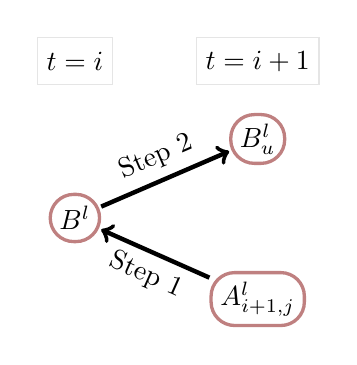
\begin{tikzpicture}
				\matrix (tree) [column sep=3em,row sep=1em,ampersand replacement=\&]{
					\node[header] (t0) {$ t = i $};  \&  \node[header] (t1) {$ t = i+1 $}; \\
					\&  \node[term] (u) {$ B^l_u $}; \\
					\node[term] (s) {$ B^l $};  \&  \\
					\&  \node[term] (d) {$ A_{i+1,j}^l $}; \\
				};
				\draw[->,ultra thick] (s) -- (u) node[midway,above,sloped] {Step 2};
				\draw[->,ultra thick] (d) -- (s) node[midway,below,sloped] {Step 1};
				\end{tikzpicture}
			\end{figure}
		\end{minipage}
	\end{frame}
	
	
	\begin{frame}{Singular points method for Asian options}{Down movement at node $ N_{i,j}, \  \forall i < n $}
		\begin{minipage}[t]{0.6\linewidth}
			\begin{enumerate}
				\item Take a singular point $ A_{i+1,j+1}^l $.
				\item $ C^l = \frac{ ( i+2) A_{i+1,j+1}^l - S_{i+1,j+1} }{ i+1 } $.
				\item Each $ C^l \in \left[ A_{i,j}^{\min}, A_{i,j}^{\max} \right] $ is a singular average of $ N_{i,j} $.
				\item For each such $ C^l $, $ C^l_d = \frac{(i+1) C^l + S_{i+1,j}}{i+2}  $
				\item $ v_{i,j}( C^l ) = \frac{1}{R} \left[ p v_{i+1,j+1} \left( A_{i+1,j+1}^l \right) + (1 - p) v_{i+1,j} \left( C^l_d \right) \right] $.
				\item $ \left( C^l, v_{i,j}( C^l ) \right) $ is singular point of $ N_{i,j} $.
			\end{enumerate}
		\end{minipage}
		\begin{minipage}[t]{0.3\linewidth}
			\begin{figure}
				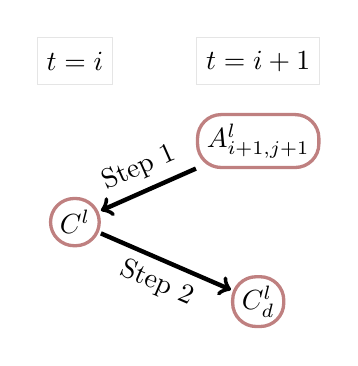
\begin{tikzpicture}
				\matrix (tree) [column sep=3em,row sep=1em,ampersand replacement=\&]{
					\node[header] (t0) {$ t = i $};  \&  \node[header] (t1) {$ t = i+1 $}; \\
					\&  \node[term] (u) {$ A_{i+1,j+1}^l $}; \\
					\node[term] (s) {$ C^l $};  \&  \\
					\&  \node[term] (d) {$ C^l_d $}; \\
				};
				\draw[->,ultra thick] (u) -- (s) node[midway,above,sloped] {Step 1};
				\draw[->,ultra thick] (s) -- (d) node[midway,below,sloped] {Step 2};
				\end{tikzpicture}
			\end{figure}
		\end{minipage}
	\end{frame}
	
	
	\begin{frame}{Singular points method for Asian options}
		\begin{block}{Aggregation and final price}
			\begin{itemize}
				\item Sort the singular points obtained according to the abscissa.
				\item Repeat the procedure for each node in a backward fashion.
				\item $ P_{0,0}^1 $ is the exact binomial price.
			\end{itemize}
		\end{block}
		\begin{block}{Introduction to approximation}
			\begin{itemize}
				\item Ability to approximate id a key strength of the method.
				\item Not all points necessary $ \implies $ selectively remove points.
				\item Net result: reduction of complexity from exponential time to polynomial time (experimental).
				\item Experimental order of complexity: $ O(n^3) $.
			\end{itemize}
		\end{block}
	\end{frame}
	
	
	\begin{frame}{Singular points method for Asian options}{Approximations: upper estimates}
		\definecolor{ffffqq}{rgb}{1.,1.,0.}
		\definecolor{dqfqcq}{rgb}{0.8156862745098039,0.9411764705882353,0.7529411764705882}
		\definecolor{wqwqwq}{rgb}{0.3764705882352941,0.3764705882352941,0.3764705882352941}
		\definecolor{afeeee}{rgb}{0.6862745098039216,0.9333333333333333,0.9333333333333333}
		\definecolor{ffffff}{rgb}{1.,1.,1.}
		\begin{tikzpicture}[line cap=round,line join=round,>=triangle 45,x=0.59cm,y=0.45cm]
		\draw[->,color=ffffff] (0.,0.) -- (17.,0.);
		\foreach \x in {,2.,4.,6.,8.,10.,12.,14.,16.}
		\draw[shift={(\x,0)},color=ffffff] (0pt,2pt) -- (0pt,-2pt);
		\draw[color=ffffff] (16.503014413215865,0.12712930521358398) node [anchor=south west] { A};
		\draw[->,color=ffffff] (0.,0.) -- (0.,13.);
		\foreach \y in {,2.,4.,6.,8.,10.,12.}
		\draw[shift={(0,\y)},color=ffffff] (2pt,0pt) -- (-2pt,0pt);
		\draw[color=ffffff] (0.158911605284918,12.306834374720044) node [anchor=west] { P};
		\clip(-1.,-1.) rectangle (17.,13.);
		\draw [line width=2.pt,color=afeeee] (16.,12.)-- (12.05,7.25);
		\draw [line width=2.pt,color=afeeee] (8.053489465238158,3.603050081817436)-- (4.,2.5);
		\draw [line width=2.pt,color=afeeee] (4.,2.5)-- (1.,2.);
		\draw [line width=0.4pt,color=wqwqwq] (12.05,7.25)-- (12.,0.);
		\draw [line width=0.4pt,color=wqwqwq] (8.053489465238158,3.603050081817436)-- (8.,0.);
		\draw [line width=0.4pt,color=wqwqwq] (4.,2.5)-- (4.,0.);
		\draw [line width=0.4pt,color=wqwqwq] (1.,2.)-- (1.,0.);
		\draw [line width=2.pt,dash pattern=on 1pt off 1pt on 2pt off 4pt,color=dqfqcq] (4.,2.5)-- (12.05,7.25);
		\draw [line width=0.4pt,color=wqwqwq] (16.,12.)-- (16.,0.);
		\draw [line width=1.2pt,dotted,color=ffffqq] (8.025,4.875)-- (8.053489465238158,3.603050081817436);
		\draw [line width=2.pt,color=afeeee] (8.053489465238158,3.603050081817436)-- (12.05,7.25);
		\draw [color=dqfqcq](2.487010827086094,9.891377575661947) node[anchor=north west] {$f_u(A) \ge f(A) \quad \forall A$};
		\draw [color=ffffqq](2.518793148143078,8.397608239402336) node[anchor=north west] {$(f_u - f)(A) \le \varepsilon \quad \forall A$};
		\begin{scriptsize}
		\draw [fill=afeeee] (16.,12.) circle (2.0pt);
		\draw[color=afeeee] (16.40766745004491,11.512276217135144) node {$S_5$};
		\draw [fill=afeeee] (12.05,7.25) circle (2.0pt);
		\draw[color=afeeee] (12.434877317921963,6.840274250535932) node {$S_4$};
		\draw [fill=afeeee] (8.053489465238158,3.603050081817436) circle (2.0pt);
		\draw[color=afeeee] (8.430304864742027,3.1217420730386003) node {$S_3$};
		\draw [fill=afeeee] (4.,2.5) circle (2.0pt);
		\draw[color=afeeee] (4.362167769448127,2.041142978723137) node {$S_2$};
		\draw[color=afeeee] (6.396236317095077,2.8039188100046406) node {f};
		\draw [fill=afeeee] (1.,2.) circle (2.0pt);
		\draw[color=afeeee] (1.4064119111486517,1.6915373893857808) node {$S_1$};
		\draw [fill=afeeee] (16.,0.) circle (2.0pt);
		\draw[color=afeeee] (16.185191202646024,-0.43787847294175086) node {$A_5$};
		\draw [fill=afeeee] (12.,0.) circle (2.0pt);
		\draw[color=afeeee] (12.117054107352125,-0.4696607992451468) node {$A_4$};
		\draw [fill=afeeee] (8.,0.) circle (2.0pt);
		\draw[color=afeeee] (8.080699333115207,-0.5332254518519388) node {$A_3$};
		\draw [fill=afeeee] (4.,0.) circle (2.0pt);
		\draw[color=afeeee] (4.04434455887829,-0.5650077781553349) node {$A_2$};
		\draw [fill=afeeee] (1.,0.) circle (2.0pt);
		\draw[color=afeeee] (1.056806379521832,-0.5332254518519388) node {$A_1$};
		\draw[color=dqfqcq] (9.002386643767732,6.109280745557824) node {$f_u$};
		\draw [fill=dqfqcq] (8.025,4.875) circle (2.0pt);
		\draw[color=dqfqcq] (7.508617554089503,5.092246303849152) node {$R_3$};
		\draw[color=ffffqq] (8.398522543685043,4.265905819960856) node {$\varepsilon_3$};
		\draw[color=afeeee] (10.464373412388976,5.314722587972924) node {f};
		\end{scriptsize}
		\end{tikzpicture}
	\end{frame}
	
	
	\begin{frame}{Singular points method for Asian options}{Approximations: lower estimates}
		\definecolor{ffffqq}{rgb}{1.,1.,0.}
		\definecolor{wqwqwq}{rgb}{0.3764705882352941,0.3764705882352941,0.3764705882352941}
		\definecolor{afeeee}{rgb}{0.6862745098039216,0.9333333333333333,0.9333333333333333}
		\definecolor{ffffff}{rgb}{1.,1.,1.}
		\begin{tikzpicture}[line cap=round,line join=round,>=triangle 45,x=0.59cm,y=0.45cm]
		\draw[->,color=ffffff] (0.,0.) -- (17.,0.);
		\foreach \x in {,2.,4.,6.,8.,10.,12.,14.,16.}
		\draw[shift={(\x,0)},color=ffffff] (0pt,2pt) -- (0pt,-2pt);
		\draw[color=ffffff] (16.983734759565976,0.15704689406799202) node [anchor=south west] { A};
		\draw[->,color=ffffff] (0.,0.) -- (0.,13.);
		\foreach \y in {,2.,4.,6.,8.,10.,12.}
		\draw[shift={(0,\y)},color=ffffff] (2pt,0pt) -- (-2pt,0pt);
		\draw[color=ffffff] (0.19630858508193877,12.246817877668772) node [anchor=west] { P};
		\clip(-1.,-1.) rectangle (17.,13.);
		\draw [line width=2.pt,color=afeeee] (4.,2.5)-- (12.,8.);
		\draw [line width=2.pt,color=afeeee] (16.,12.)-- (12.,8.);
		\draw [line width=0.4pt,color=wqwqwq] (12.,8.)-- (12.,0.);
		\draw [line width=0.4pt,color=wqwqwq] (4.,2.5)-- (4.,0.);
		\draw [line width=0.4pt,color=wqwqwq] (1.,2.)-- (1.,0.);
		\draw [line width=2.pt,dash pattern=on 2pt off 2pt,color=afeeee] (4.,2.5)-- (7.,3.);
		\draw [line width=2.pt,dash pattern=on 2pt off 2pt,color=afeeee] (12.,8.)-- (7.,3.);
		\draw [line width=0.4pt,color=wqwqwq] (7.,3.)-- (6.998942733420039,0.);
		\draw [line width=0.4pt,color=wqwqwq] (16.,12.)-- (16.,0.);
		\draw [line width=1.2pt,dash pattern=on 1pt off 1pt,color=ffffqq] (7.000519372007349,4.562857068255052)-- (7.,3.);
		\draw [color=afeeee](1.9857588593058553,11.540106854362808) node[anchor=north west] {$f_d(A) \le f(A) \quad \forall A$};
		\draw [color=ffffqq](1.9857588593058553,10.48004031940386) node[anchor=north west] {$(f - f_d) (A) \le \delta  \quad  \forall A$};
		\draw [line width=2.pt,color=afeeee] (1.,2.)-- (4.,2.5);
		\begin{scriptsize}
		\draw [fill=afeeee] (16.,12.) circle (2.0pt);
		\draw[color=afeeee] (16.355547287303775,11.500845130845809) node {$S_4$};
		\draw [fill=afeeee] (12.,8.) circle (2.0pt);
		\draw[color=afeeee] (12.429375585664998,7.260578991010025) node {$S_3$};
		\draw [fill=afeeee] (4.,2.5) circle (2.0pt);
		\draw[color=afeeee] (4.4592470313382835,2.03876976324929) node {$S_2$};
		\draw [fill=afeeee] (1.,2.) circle (2.0pt);
		\draw[color=afeeee] (1.2790479530108758,1.5283673575283159) node {$S_1$};
		\draw [fill=afeeee] (16.,0.) circle (2.0pt);
		\draw[color=afeeee] (16.041453551172673,-0.7095508829405706) node {$A_4$};
		\draw [fill=afeeee] (12.,0.) circle (2.0pt);
		\draw[color=afeeee] (12.076020132517508,-0.6702891594235725) node {$A_3$};
		\draw [fill=afeeee] (4.,0.) circle (2.0pt);
		\draw[color=afeeee] (4.105891578190794,-0.6702891594235725) node {$A_2$};
		\draw [fill=afeeee] (1.,0.) circle (2.0pt);
		\draw[color=afeeee] (1.0042159338961614,-0.7488126064575684) node {$A_1$};
		\draw [fill=afeeee] (6.998942733420039,0.) circle (2.0pt);
		\draw[color=afeeee] (7.011258637403488,-0.7095508829405706) node {$A_{23}$};
		\draw [fill=afeeee] (7.,3.) circle (2.0pt);
		\draw[color=afeeee] (7.482399241600141,2.156554933800284) node {$R_{23}$};
		\draw[color=afeeee] (5.833407126911855,2.156554933800284) node {$f_d$};
		\draw[color=afeeee] (9.798840545567018,4.9441373035071425) node {$f_d$};
		\draw [fill=afeeee] (7.000519372007349,4.562857068255052) circle (2.0pt);
		\draw[color=afeeee] (6.5793797502232225,5.925680391432093) node {$S_{23}$};
		\draw[color=ffffqq] (7.286090656518202,3.7270238744802042) node {$\delta_4$};
		\end{scriptsize}
		\end{tikzpicture}
	\end{frame}
	
	
	\begin{frame}{Singular points method for Asian options}{Numerical results}
		Data: $ s_0 = 100, T = 1, r = 0.1, q = 0.03 $.
		\begin{tabular}{crcccc}
			\toprule
			&         &  \multicolumn{2}{c}{$ K = 90 $}  &  \multicolumn{2}{c}{$ K = 110 $}  \\
			\cmidrule(lr){3-4}\cmidrule(lr){5-6}
			&  $ n $  &  $ \sigma = 0.2 $  &  $ \sigma = 0.4 $  &  $ \sigma = 0.2 $  &  $ \sigma = 0.4 $  \\
			\midrule
			\multirow{2}{2em}{Bin}
			&   10  &  14.5912  &  17.8033  &  2.5100  &  6.6523  \\
			&   25  &  15.1535  &  18.6786  &  2.6270  &  7.3451  \\
			\midrule
			\multirow{6}{2em}{SP}
			&   10  &  14.5925  &  17.8068  &  2.5090  &  6.6511  \\
			&   25  &  15.1535  &  18.6785  &  2.6270  &  7.3449  \\
			&   50  &  15.3524  &  19.0420  &  2.6673  &  7.4563  \\
			&  100  &  15.4732  &  19.2696  &  2.6886  &  7.5174  \\
			&  200  &  15.5453  &  19.4065  &  2.6996  &  7.5502  \\
			&  400  &  15.5861  &  19.4845  &  2.7053  &  7.5674  \\
			\bottomrule
		\end{tabular}
	\end{frame}
	
	
	\begin{frame}{Singular points method for Asian options}{Summary}
		\begin{itemize}
			\neu Introduced by Gaudenzi \emph{et al} \cite{Gaudenzi2010} in 2010.
			\pro Convergent to exact CRR and thus BS.
			\pro Approximation -- \emph{A priori} error bounds.
			\pro Fast -- experimental order of complexity $ O(n^3) $.
			\con Difficult to compute theoretical complexity.
			\con Depends on the recombinant nature of the underlying's tree.
			\con<alert@1-> Not extensible to GM, since the price function is non-linear. $ G_u = \left( G^{i+1} S_{i+1,j} \right)^{\frac{1}{i+2}} \propto G^{\frac{i+1}{i+2}} $
			\con<alert@1-> Assumes constant volatility, hence not applicable to local volatility models.
		\end{itemize}
	\end{frame}
	
	
	
	\section{Cliquet options}
	
	\begin{frame}[allowframebreaks]{Cliquet options: introduction}
		\begin{description}
			\item[forward start option] An option that starts at a future date $ u $, with an expiration date $ T $ set further in the future. The payoff is given by $ (S_T - S_u)_+ $.
			\item[cliquet option] An exotic option consisting of a series of consecutive at-the-money forward start options, where the return may be locally or globally capped and floored.
		\end{description}
		\begin{block}{Pros and cons}
			\begin{itemize}
				\pro Safety against downside risks.
				\pro Significant upside potential.
				\con Unbounded gains not possible.
			\end{itemize}
		\end{block}
		\begin{block}{Some terminology}
			\begin{itemize}
				\item Observation times: time points at which one forward start option expires, and another starts. Assumption: observation times are equidistant.
				\item Return: $ R_i = \frac{S_i - S_{i-1}}{S_{i-1}} = \frac{S_i}{S_{i-1}} - 1 $.
				\item Running sum: $ Z_i = \sum_{k = 1}^{i} \max \{ F_{loc}, \min \{ C_{loc}, R_k \} \} $.
				\item $ \mathrm{Payoff} = \mathrm{notional} \cdot \max \{ F_{glob}, \min \{ C_{glob}, Z_{N} \} \} $.
			\end{itemize}
		\end{block}
		\begin{block}{Pre-existing methods for pricing cliquet options}
			\begin{itemize}
				\item No prominent tree-based method.
				\item \cite{Wilmott2002}: PDE based, FD approach.
				\item \cite{Windcliff2006}: PDE based, FD approach; many more generalisations.
			\end{itemize}
		\end{block}
	\end{frame}
	
	
	\begin{frame}{Singular points method for cliquet options}{Introduction}
		Idea: At every observational time $ i $: 
		\begin{itemize}
			\item The possible paths are $ 2^m $, where $ m $ is the number of steps in each duration.
			\item The probability of choosing a path is binomially distributed.
			\item The running sums $ Z $ depend on the possible paths and respective probabilities.
		\end{itemize}
		Start with maturity, and proceed backwards.
	\end{frame}
	
	
	\begin{frame}{Singular points method for cliquet options}{At maturity ($ i = N $)}
		The price function is not convex, but is piecewise-linear and continuous. It is characterised by four singular points, as depicted in the figure below.
		
		\definecolor{wqwqwq}{rgb}{0.3764705882352941,0.3764705882352941,0.3764705882352941}
		\definecolor{afeeee}{rgb}{0.6862745098039216,0.9333333333333333,0.9333333333333333}
		\definecolor{dqfqcq}{rgb}{0.8156862745098039,0.9411764705882353,0.7529411764705882}
		\definecolor{ffffff}{rgb}{1.,1.,1.}
		\begin{tikzpicture}[line cap=round,line join=round,>=triangle 45,x=1.0cm,y=1.0cm]
		\draw[->,color=ffffff] (0.,0.) -- (9.,0.);
		\foreach \x in {,1.,2.,3.,4.,5.,6.,7.,8.}
		\draw[shift={(\x,0)},color=ffffff] (0pt,2pt) -- (0pt,-2pt);
		\draw[color=ffffff] (8.778132976577169,0.054247335995569544) node [anchor=south west] { Z};
		\draw[->,color=ffffff] (0.,0.) -- (0.,5.);
		\foreach \y in {,1.,2.,3.,4.}
		\draw[shift={(0,\y)},color=ffffff] (2pt,0pt) -- (-2pt,0pt);
		\draw[color=ffffff] (0.06780919373316127,4.698691618151926) node [anchor=west] { P};
		\clip(-1.,-1.) rectangle (9.,5.);
		\draw [line width=2.pt,color=dqfqcq] (1.,1.)-- (2.,1.);
		\draw [line width=2.pt,color=dqfqcq] (2.,1.)-- (7.,4.);
		\draw [line width=2.pt,color=dqfqcq] (7.,4.)-- (8.,4.);
		\draw [line width=0.4pt,color=wqwqwq] (1.,1.)-- (1.,0.);
		\draw [line width=0.4pt,color=wqwqwq] (2.,1.)-- (2.,0.);
		\draw [line width=0.4pt,color=wqwqwq] (7.,4.)-- (7.,0.);
		\draw [line width=0.4pt,color=wqwqwq] (8.,4.)-- (8.,0.);
		\draw [line width=0.4pt,color=wqwqwq] (1.,1.)-- (0.,1.);
		\draw [line width=0.4pt,color=wqwqwq] (7.,4.)-- (0.,4.);
		\begin{scriptsize}
		\draw [fill=dqfqcq] (1.,1.) circle (2.5pt);
		\draw[color=dqfqcq] (0.9258283422770947,1.443851458417754) node {$S_1$};
		\draw [fill=dqfqcq] (2.,1.) circle (2.5pt);
		\draw[color=dqfqcq] (1.7666623445682943,1.443851458417754) node {$S_2$};
		\draw [fill=dqfqcq] (7.,4.) circle (2.5pt);
		\draw[color=dqfqcq] (7.204959681967828,3.613744898240536) node {$S_3$};
		\draw [fill=dqfqcq] (8.,4.) circle (2.5pt);
		\draw[color=dqfqcq] (8.18141207172535,3.6544304002372128) node {$S_4$};
		\draw [fill=afeeee] (1.,0.) circle (1.5pt);
		\draw[color=afeeee] (0.573220534864656,-0.31918696143825614) node {$F_{loc} N_{obs}$};
		\draw [fill=afeeee] (2.,0.) circle (1.5pt);
		\draw[color=afeeee] (2.2548885394470557,-0.31918696143825614) node {$F_{glob}$};
		\draw [fill=afeeee] (7.,0.) circle (1.5pt);
		\draw[color=afeeee] (6.526867744636215,-0.31918696143825614) node {$C_{glob}$};
		\draw [fill=afeeee] (8.,0.) circle (1.5pt);
		\draw[color=afeeee] (8.113602877992188,-0.3463106294360409) node {$C_{loc} N_{obs}$};
		\draw [fill=afeeee] (0.,1.) circle (1.5pt);
		\draw[color=afeeee] (-0.0506240474804277,0.73863609047535) node {$F_{glob}$};
		\draw [fill=afeeee] (0.,4.) circle (1.5pt);
		\draw[color=afeeee] (-0.07774772497369223,3.7358014042305676) node {$C_{glob}$};
		\end{scriptsize}
		\end{tikzpicture}
	\end{frame}
	
	
	\begin{frame}{Singular points method for cliquet options}{At all other times ($ i < N $)}
		Not all paths are possible due to local floors and caps. The realizable paths and associated quantities are denoted by primed variables.
		\begin{enumerate}
			\item From all the singular points $ Z_{i+1}^l $, subtract all the possible returns $ R_j' $ to get $ B_{l,j} $.
			\item Each $ B_{l,j} \in [ i F_{loc}, i C_{loc} ] $ becomes a singular point at time $ i $.
			\item The corresponding price function is: $ V_i (B_{l,j}) = e^{- \frac{rT}{N}} \sum_{j=0}^{j_0} \left[ p_j' V_{i+1} (Z + R_j') \right] $.
			\item Linear combination of piecewise-linear continuous functions is piecewise-linear continuous functions. Thus, the process may be continued.
		\end{enumerate}
		We start from maturity and go backwards. At time 0, there is only one singular point, whose ordinate is the exact binomial price.
	\end{frame}
	
	
	\begin{frame}{Singular points method for cliquet options}{Evaluation of the exact binomial price}
		Not all paths are possible due to local floors and caps. The realizable paths and associated quantities are denoted by primed variables.
		\begin{enumerate}
			\item From all the singular points $ Z_{i+1}^l $, subtract all the possible returns $ R_j' $ to get $ B_{l,j} $.
			\item Each $ B_{l,j} \in [ i F_{loc}, i C_{loc} ] $ becomes a singular point at time $ i $.
			\item The corresponding price function is: $ V_i (B_{l,j}) = e^{- \frac{rT}{N}} \sum_{j=0}^{j_0} \left[ p_j' V_{i+1} (Z + R_j') \right] $.
			\item Linear combination of piecewise-linear continuous functions is piecewise-linear continuous functions. Thus, the process may be continued.
		\end{enumerate}
		We start from maturity and go backwards. At time 0, there is only one singular point, whose ordinate is the exact binomial price.
	\end{frame}
	
	
	\begin{frame}{Singular points method for cliquet options}{Approximation}
		\definecolor{ffffqq}{rgb}{1.,1.,0.}
		\definecolor{qqffqq}{rgb}{0.,1.,0.}
		\definecolor{wqwqwq}{rgb}{0.3764705882352941,0.3764705882352941,0.3764705882352941}
		\definecolor{eqeqeq}{rgb}{0.8784313725490196,0.8784313725490196,0.8784313725490196}
		\definecolor{dqfqcq}{rgb}{0.8156862745098039,0.9411764705882353,0.7529411764705882}
		\definecolor{afeeee}{rgb}{0.6862745098039216,0.9333333333333333,0.9333333333333333}
		\definecolor{ffffff}{rgb}{1.,1.,1.}
		\begin{tikzpicture}[line cap=round,line join=round,>=triangle 45,x=0.8cm,y=0.8cm]
		\draw[->,color=ffffff] (0.,0.) -- (12.,0.);
		\foreach \x in {,1.,2.,3.,4.,5.,6.,7.,8.,9.,10.,11.}
		\draw[shift={(\x,0)},color=ffffff] (0pt,2pt) -- (0pt,-2pt);
		\draw[color=ffffff] (11.72949600014192,0.0665249798016828) node [anchor=south west] { Z};
		\draw[->,color=ffffff] (0.,0.) -- (0.,8.);
		\foreach \y in {,1.,2.,3.,4.,5.,6.,7.}
		\draw[shift={(0,\y)},color=ffffff] (2pt,0pt) -- (-2pt,0pt);
		\draw[color=ffffff] (0.08315628750088702,7.641135707448683) node [anchor=west] { P};
		\clip(-1.,-1.) rectangle (12.,8.);
		\draw [line width=2.pt,color=dqfqcq] (1.,1.)-- (2.,1.);
		\draw [line width=1.6pt,dash pattern=on 1pt off 2pt on 3pt off 4pt,color=eqeqeq] (2.,1.)-- (3.,1.75);
		\draw [line width=1.6pt,dash pattern=on 1pt off 2pt on 3pt off 4pt,color=eqeqeq] (3.,1.75)-- (4.,2.);
		\draw [color=wqwqwq] (1.,1.)-- (1.,0.);
		\draw [color=wqwqwq] (2.,1.)-- (2.,0.);
		\draw [color=wqwqwq] (3.,1.75)-- (3.,0.);
		\draw [color=wqwqwq] (4.,2.)-- (4.,0.);
		\draw [color=wqwqwq] (1.,1.)-- (0.,1.);
		\draw [line width=1.6pt,dash pattern=on 1pt off 2pt on 3pt off 4pt,color=eqeqeq] (4.,2.)-- (6.,2.75);
		\draw [line width=1.6pt,dash pattern=on 1pt off 2pt on 3pt off 4pt,color=eqeqeq] (8.,4.)-- (9.,5.);
		\draw [line width=2.pt,color=dqfqcq] (9.,5.)-- (10.,7.);
		\draw [color=wqwqwq] (6.,2.75)-- (6.,0.);
		\draw [color=wqwqwq] (9.,5.)-- (9.,0.);
		\draw [color=wqwqwq] (11.,7.)-- (11.,0.);
		\draw [line width=1.6pt,dash pattern=on 1pt off 2pt on 3pt off 4pt,color=eqeqeq] (6.,2.75)-- (8.,4.);
		\draw [color=wqwqwq] (8.,4.)-- (8.,0.);
		\draw [color=wqwqwq] (10.,7.)-- (10.,0.);
		\draw [line width=2.pt,color=dqfqcq] (10.,7.)-- (11.,7.);
		\draw [line width=2.pt,color=dqfqcq] (2.,1.)-- (9.,5.);
		\draw [line width=1.6pt,dash pattern=on 3pt off 3pt,color=afeeee] (2.,1.)-- (10.,7.);
		\draw [line width=1.6pt,dotted,color=qqffqq] (6.004094596374262,3.288054055071007)-- (6.,2.75);
		\draw [color=wqwqwq] (10.,7.)-- (0.,7.);
		\draw [line width=1.6pt,dotted,color=ffffqq] (7.999695997451529,5.499771998088647)-- (8.,4.);
		\draw [color=qqffqq](1.0023349125274963,6.194217396762082) node[anchor=north west] {$| (V_1 - V)(Z) | \le h  \quad  \forall Z$};
		\draw [color=ffffqq](1.0023349125274963,5.19634269973684) node[anchor=north west] {$\exists Z \: | (V_2 - V)(Z) | > h$};
		\begin{scriptsize}
		\draw [fill=afeeee] (1.,1.) circle (2.0pt);
		\draw[color=afeeee] (0.9857036550273188,1.3877876060904992) node {$S_1$};
		\draw [fill=afeeee] (2.,1.) circle (2.0pt);
		\draw[color=afeeee] (1.8338977875363665,1.4376813409417613) node {$S_2$};
		\draw [fill=afeeee] (3.,1.75) circle (2.0pt);
		\draw[color=afeeee] (2.9149295250478975,2.0862998940081687) node {$S_3$};
		\draw [fill=afeeee] (4.,2.) circle (2.0pt);
		\draw[color=afeeee] (4.212167610061735,1.6705187702476512) node {$S_4$};
		\draw [fill=afeeee] (1.,0.) circle (2.0pt);
		\draw[color=afeeee] (0.9191786250266092,-0.35849311370367437) node {$Z_1$};
		\draw [fill=afeeee] (2.,0.) circle (2.0pt);
		\draw[color=afeeee] (1.9503165900376083,-0.3252306238028329) node {$Z_2$};
		\draw [fill=afeeee] (3.,0.) circle (2.0pt);
		\draw[color=afeeee] (2.9481920400482524,-0.3252306238028329) node {$Z_3$};
		\draw [fill=afeeee] (4.,0.) circle (2.0pt);
		\draw[color=afeeee] (3.929436232558719,-0.35849311370367437) node {$Z_4$};
		\draw [fill=afeeee] (0.,1.) circle (2.0pt);
		\draw[color=afeeee] (0.037721977517206906,0.7558002979745126) node {$F_{glob}$};
		\draw [fill=afeeee] (0.,7.) circle (2.0pt);
		\draw[color=afeeee] (0.004459462516852086,6.7264172351755445) node {$C_{glob}$};
		\draw [fill=afeeee] (6.,2.75) circle (2.0pt);
		\draw[color=afeeee] (6.174655995082668,2.302506078363638) node {$S_5$};
		\draw [fill=afeeee] (8.,4.) circle (2.0pt);
		\draw[color=afeeee] (8.15377563760378,3.5997431844964525) node {$S_6$};
		\draw [fill=afeeee] (9.,5.) circle (2.0pt);
		\draw[color=afeeee] (9.218176117615133,4.597617881521694) node {$S_7$};
		\draw [fill=afeeee] (10.,7.) circle (2.0pt);
		\draw[color=afeeee] (10.166157795125246,6.560104785671337) node {$S_8$};
		\draw [fill=afeeee] (11.,7.) circle (2.0pt);
		\draw[color=afeeee] (11.197295760136244,6.576736030621758) node {$S_9$};
		\draw [fill=afeeee] (6.,0.) circle (2.0pt);
		\draw[color=afeeee] (5.9584496475803626,-0.30859937885241223) node {$Z_5$};
		\draw [fill=afeeee] (8.,0.) circle (2.0pt);
		\draw[color=afeeee] (7.95420054760165,-0.3252306238028329) node {$Z_6$};
		\draw [fill=afeeee] (9.,0.) circle (2.0pt);
		\draw[color=afeeee] (8.952075997612294,-0.3418618687532536) node {$Z_7$};
		\draw [fill=afeeee] (11.,0.) circle (2.0pt);
		\draw[color=afeeee] (10.89793312513305,-0.3418618687532536) node {$Z_9$};
		\draw [fill=afeeee] (10.,0.) circle (2.0pt);
		\draw[color=afeeee] (9.933320190122762,-0.3252306238028329) node {$Z_8$};
		\draw[color=dqfqcq] (6.540543660086572,3.8658431037031837) node {$V_1$};
		\draw[color=afeeee] (5.559299467576104,3.9822618183561285) node {$V_2$};
		\draw [color=qqffqq] (6.004094596374262,3.288054055071007)-- ++(-2.0pt,-2.0pt) -- ++(4.0pt,4.0pt) ++(-4.0pt,0) -- ++(4.0pt,-4.0pt);
		\draw[color=qqffqq] (6.340968570084443,3.0841745910334106) node {$\le$ h};
		\draw [color=ffffqq] (7.999695997451529,5.499771998088647)-- ++(-1.5pt,-1.5pt) -- ++(3.0pt,3.0pt) ++(-3.0pt,0) -- ++(3.0pt,-3.0pt);
		\draw[color=ffffqq] (8.303456955105375,4.847086555778005) node {>h};
		\end{scriptsize}
		\end{tikzpicture}
	\end{frame}
	
	
	%\begin{frame}{Singular points method for cliquet options}{Numerical results}
	%	Data: $ F_{loc} = 0, C_{loc} = 0.08, F_{glob} = 0.16 $, $ C_{glob} = \infty, T = 5, N = 5, r = 0.03 $.
	%	\begin{tabular}{rrcccc}
	%		\toprule
	%		\multirow{2}{1em}{$ \sigma $}  &  \multirow{2}{1em}{$ m $}
	%		&  \multicolumn{2}{c}{Price}  &  \multicolumn{2}{c}{Time (s)\tablefootnote{$ \infty $ means time taken is more than an hour.}}  \\
	%		\cmidrule(lr){3-5}\cmidrule(lr){6-7}
	%		&&  Bin  &  SP  &  Bin  &  SP  \\
	%		\midrule
	%		\multirow{3}{2em}{$ 0.2 $}
	%		&   200  &  0.173716366  &  0.173716366  &  0.0165  &  0.00828  \\
	%		&   500  &  0.173922597  &  0.173922671  &  0.0875  &  0.0437  \\
	%		&  1000  &  0.174051949  &  0.174051983  &  2.38  &  0.183  \\
	%		\midrule
	%		\multirow{3}{2em}{$ 0.02 $}
	%		&   200  &  0.150465004  &  0.150466828  &  600  &  6.09  \\
	%		&   500  &  0.150508871  &  0.150510526  &  $ \infty $  &  24.2  \\
	%		&  1000  &  0.150522368  &  0.150524027  &  $ \infty $  &  55  \\
	%		\bottomrule
	%	\end{tabular}	
	%\end{frame}
	
	
	\begin{frame}{Singular points method for cliquet options}{Experimental computational complexity -- $ O(m^2) $}
		% This plot was generated by plotly
		\begin{figure}
			\centering
			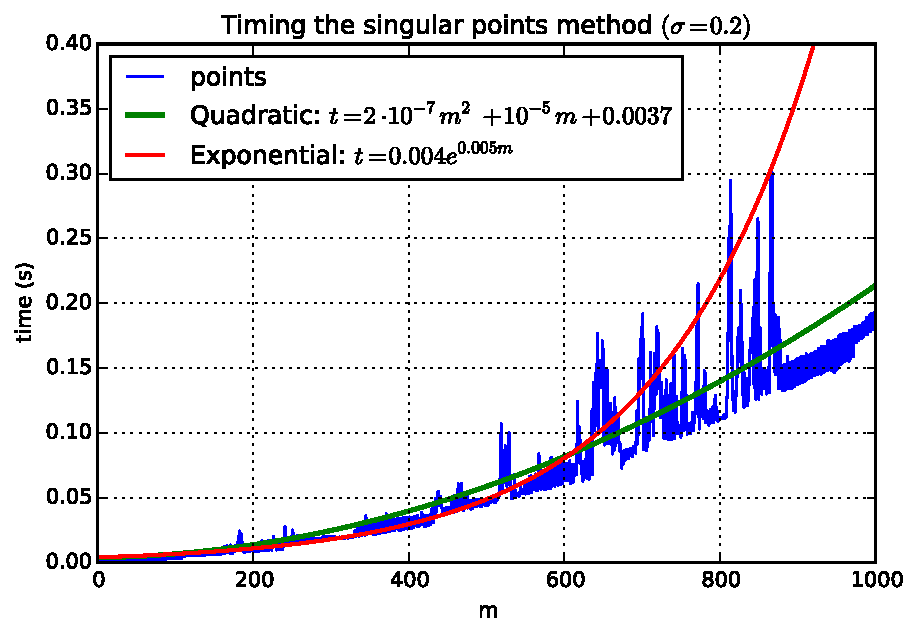
\includegraphics[width=0.85\linewidth]{../img/timing-cliquet}
		\end{figure}
	\end{frame}
	
	
	\begin{frame}{Singular points method for cliquet options}{Summary}
		\begin{itemize}
			\neu Introduced by Gaudenzi \emph{et al} \cite{Gaudenzi2011} in 2011.
			\pro Convergent to exact CRR and thus BS.
			\pro Approximation -- \emph{A priori} error bounds.
			\pro Significant speed improvement in low volatility cases against binomial model.
			\pro<alert@1-> Can be used for local volatility models and varying interest rates in each period.
			\pro<alert@1-> Fast -- experimental order of complexity $ O(m^2) $.
			\con Difficult to compute theoretical complexity.
		\end{itemize}
	\end{frame}
	
	
	\section{Conclusion}
	
	\begin{frame}{Recapitulation}
		\begin{itemize}
			\item The singular points method is a new efficient technique to evaluate path-dependent exotic options.
			\item The theory varies with option type.
			\item In the Asian case, the method is quite complicated and is not very flexible, although it is fast and efficient. It is easily generalised to the American case and to lookback options. \alert{We have shown that it fails to be generalised for geometric mean and local volatility models.}
			\item In the cliquet case, the method is quite flexible, and takes care of local volatility models and varying interest rates. \alert{We have found out that the experimental order of computational complexity is approximately $ O(m^2) $ for low $ m $}, which is a marked improvement over pre-existing methods.
		\end{itemize}
	\end{frame}
	
	
	\begin{frame}{Further research}
		\begin{itemize}
			\item Theoretical complexity: dependence of singular point redundancy on initial data.
			\item Customising the method for other path-dependent options (like?).
		\end{itemize}
	\end{frame}
	
	
	\begin{frame}[plain,c]
		%\frametitle{A first slide}
		
		\begin{center}
			{\Huge Questions?}
		\end{center}
		
		\vfill
		
		\begin{center}
			{\Huge Thank you!}
		\end{center}
		
	\end{frame}
	
	
	\appendix
	%\section<presentation>*{\appendixname}
	%\subsection<presentation>*{Bibliography}
	
	\begin{frame}[allowframebreaks]
		\frametitle<presentation>{Bibliography}
		\printbibliography
	\end{frame}
	
	
\end{document}
